\documentclass[10pt]{article}

\def\HandoutNumber{3}
\def\TheDate{February 12, 2016}
\def\Name{Blake Riley}

\usepackage{amsmath,amsfonts,amsthm,amssymb}
\usepackage{setspace}
\usepackage{graphicx,float,wrapfig}
%\usepackage{parskip}
\usepackage{enumerate}
\usepackage{url}

\usepackage{fourier}
\usepackage[T1]{fontenc}
\usepackage[protrusion=true,expansion=true]{microtype}

% In case you need to adjust margins:
\topmargin=-0.45in      %
\evensidemargin=0in     %
\oddsidemargin=0in      %
\textwidth=6.5in        %
\textheight=9.0in       %
\headsep=0.25in         %
\parindent=0in

\usepackage[nodayofweek]{datetime} \usdate
% Pdf metadata
\pdfinfo{  /Author (\Name)
           /Title (Economics 533 Handout \HandoutNumber)
           /Keywords ()
           /ModDate (D:\pdfdate)}

\newtheoremstyle{basic}% name
   {5pt}% Space above
   {5pt}% Space below
   {\itshape \leftskip=1em}% Body font
   {-1em}% Indent amount
   {\bfseries}% Theorem head font
   {:}% Punctuation after theorem head
   { }% Space after theorem head
   {}% Theorem head spec (can be left empty, meaning `normal')
\theoremstyle{basic}
\newtheorem{exercise}{Exercise}[]
\newtheorem{definition}{Definition}[section]
\newtheorem{theorem}{Theorem}[section]
\newtheorem{lemma}[theorem]{Lemma}

\usepackage{tikz} % For drawing diagrams
\usetikzlibrary{calc}
\tikzset{
% Two node styles for game trees: solid and hollow
solid node/.style={circle,draw,inner sep=1.5,fill=black},
hollow node/.style={circle,draw,inner sep=1.5}
}

%%%%%%%%%%%%%%%%%%%%%%%%%%%%%%%%%%%%%%%%%%%%%%%%%%%%%%%%%%%%

% Custom commands

\newcommand{\R}{\mathbb{R}}
\newcommand{\N}{\mathbb{N}}
\newcommand{\E}{\operatorname{E}}
\renewcommand{\P}{\operatorname{Pr}}
\newcommand{\Var}{\operatorname{Var}}
\newcommand{\Cov}{\operatorname{Cov}}
\newcommand{\cond}{\,|\,}
\newcommand{\bigcond}{\;\big|\;}
\newcommand{\argmax}{\mathop{\operatorname{arg\,max}}}
\newcommand{\noti}{{{\scriptscriptstyle-}\!i}}
\newcommand{\notj}{{{\scriptscriptstyle-}\!j}}
\newcommand{\notij}{{{\scriptscriptstyle-}\!\{i,j\}}}
\newcommand{\I}{\mathbb{I}}
\newcommand{\tto}{\twoheadrightarrow}


%%%%%%%%%%%%%%%%%%%%%%%%%%%%%%%%%%%%%%%%%%%%%%%%%%%%%%%%%%%%%
%%%%%%%%%% The main document content
%%%%%%%%%%%%%%%%%%%%%%%%%%%%%%%%%%%%%%%%%%%%%%%%%%%%%%%%%%%%%

\begin{document}
\begin{spacing}{1.0}

\noindent
\textbf{Handout \HandoutNumber} \\
Econ 533 \\
\TheDate \\
TA: \Name \\

\section{Finitely repeated games}

Unsurprisingly, in repeated games we're analyzing a
specific game (such as the prisoners' dilemma, battle of
the sexes, etc) that is played over and over again in a
supergame. At each stage of the repetition, let $G$
denote a static game of complete information in which the
players involved choose their corresponding actions
simultaneously. The game $G$ will then be called the
\textbf{stage game} of the full game.

\begin{definition}
  Given a stage game $G$, let $G(T)$ denote the finitely
  repeated game in which $G$ is played $T<\infty$ times,
  with the outcomes of all preceding plays observed
  before the next play begins. The payoffs of $G(T)$ are
  simply the sum of the payoffs for each of the $T$ stages.
\end{definition}

\begin{theorem}
  If the stage game $G$ has a unique Nash equilibrium,
  then for all finite $T$, the repeated game $G(T)$ has a
  unique subgame-perfect outcome where the unique NE is
  played at every stage.
\end{theorem}

If there are multiple equilibria at every
stage, then there might be subgame-perfect NEs that do
not involve playing ``stage-game equilibrium
strategies''.

\section{Infinitely repeated games}

In finitely repeated games, there might be credible threats that influence
current behavior if the stage game has multiple equilibria. A stronger
result can be stated for the infinitely repeated case: even if the stage
game has a unique NE, there might be subgame-perfect NEs of the infinitely
repeated game in which no choice of actions at any stage is a NE of $G$.

\begin{definition}
  Given a stage game $G$, let $G(\infty, \delta)$ denote
  the infinitely repeated game in which $G$ is repeated
  indefinitely and players share the discount factor
  $\delta$. For each $t$, the outcomes the the $t-1$
  preceding plays are observed before the stage
  begins. The payoffs of each player are the present
  values of the sequence of payoffs from the stage games.
\end{definition}

\subsection{Payoffs}
 In contrast to simply summing up payoffs like in the
 finitely repeated games, we're now discounting future
 payoffs to make the near future more salient and to keep
 things tractable. Given a discount factor $\delta$ and a
 sequence of payoffs $\{\pi_t^i\}_{t=1}^\infty$ to player
 $i$, the total payoff is
 $\pi_1^i+\delta\pi_2^i+\delta^2\pi_3^i+\ldots = \sum
 \delta^{t-1} \pi_t$. Occasionally this is rescaled by
 $1-\delta$ so we get rid of this factor when stage game
 payoffs are identical across all periods.

 The discount factor $\delta$ can often be interpreted as either a
time-discount factor or a fixed probability that the game ends at that stage.


\subsection{Folk theorems}

A ``folk theorem'' is a name for any theorem that is generally known, but
not necessesarily attributable to any individual. In the context of
repeated games, ``the folk theorem'' is a general feasibility theorem that
says a very large range of payoffs are acheivable in a Nash equilibrium of
an infinitely repeated game. Many further extensions exist for folk
theorems when agents have incomplete information and actions are only
partially observable.

\begin{definition}
  In an $n$-player game, call the vector $(x_1,\ldots,
  x_n)$ a \emph{feasible vector} in stage game $G$ if each $x_i$
  is a convex combination of the pure-strategy payoffs of $G$.
\end{definition}

\begin{definition}
  A payoff vector $(x_1, \ldots, x_n)$ is \emph{enforceable} if, for all $i$, the
  payoff $x_i$ is at least the minimum payoff other players can force on $i$:
  \begin{align*}
    x_i \ge m_i = \min_{s_\noti} \max_{s_i} \pi_i(s_i, s_\noti)
  \end{align*}
\end{definition}

\begin{theorem}
  (``The Folk Theorem'') Let $G$ be a finite, static game of complete
  information with $n$ players, and let $(x_1, \ldots, x_n)$ be a feasible
  and enforceable payoff vector. Then there exists a Nash equilibrium of
  $G(\infty, \delta)$ that acheives $x$ as payoffs if $\delta$ is
  sufficiently close to one.
\end{theorem}

\begin{theorem}
  (Friedman 1971) Let $G$ be a finite, static game of
  complete information with $n$ players. Let $(e_1,
  \ldots, e_n)$ be the payoffs from a Nash equilibrium of
  $G$, and let $(x_1, \ldots, x_n)$ be any other feasible
  payoffs from $G$. If $x_1 > e_i$ for each player $i$
  and $\delta$ is sufficiently close to one, then there
  exists a subgame-perfect Nash equilibrium of the
  infinitely repeated game $G(\infty, \delta)$ that
  achieves $(x_1, \ldots, x_n)$ as payoffs.
\end{theorem}

\begin{theorem}
  (Aumann and Shapley 1976, Rubinstein 1979) Even without discounting,
  every feasible and enforceable vector of payoffs is achievable in a
  subgame perfect Nash equilibrium.
\end{theorem}

\newpage
\section{Exercises}

\begin{exercise}
  Find all WPNEs and sequential equilibria:
  \begin{center}
    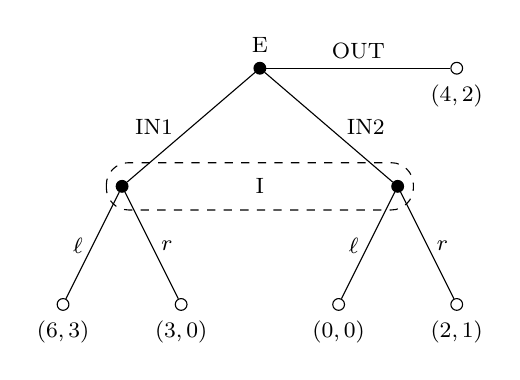
\begin{tikzpicture}[scale=1,font=\footnotesize]
      % Specify spacing for each level of the tree
      \tikzstyle{level 1}=[level distance=15mm,sibling distance=35mm]
      \tikzstyle{level 2}=[level distance=15mm,sibling distance=15mm]
      % The Tree
      \node(0)[solid node,label=above:{E}]{}
      child[missing] % Missing very left node to balance tree
      % Actual left node
      child{node(1)[solid node]{} child{node[hollow node,label=below:{$(6,3)$}]{}
          edge from parent node[left]{$\ell$} } child{node[hollow
          node,label=below:{$(3,0)$}]{} edge from parent node[right]{$r$} } edge from
        parent node[left,xshift=-3]{IN1} }
      % Right node
      child{node(2)[solid node]{} child{node[hollow node,label=below:{$(0,0)$}]{}
          edge from parent node[left]{$\ell$} coordinate[pos=.8] (l)}
        child{node[hollow node,label=below:{$(2,1)$}]{} edge from parent
          node[right]{$r$} coordinate[pos=.8] (r)} edge from parent
        node[right,xshift=3]{IN2} }
      % Right branch
      child[grow=right, level distance = 25mm]{
        node[hollow node, label=below:{$(4,2)$}]{} edge from parent node[above]{OUT}
      } ;
      % information set
      \draw[dashed,rounded corners=8]($(1) + (-.2,.3)$)rectangle($(2) +(.2,-.3)$);
      % specify mover at 2nd information set
      \node at ($(1)!.5!(2)$) {I};
    \end{tikzpicture}
  \end{center}
\end{exercise}

\begin{exercise}
  Find all WPNEs and sequential equilibria:
  \begin{center}
    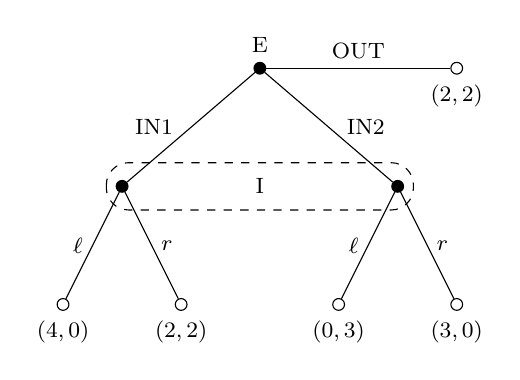
\begin{tikzpicture}[scale=1,font=\footnotesize]
      % Specify spacing for each level of the tree
      \tikzstyle{level 1}=[level distance=15mm,sibling distance=35mm]
      \tikzstyle{level 2}=[level distance=15mm,sibling distance=15mm]
      % The Tree
      \node(0)[solid node,label=above:{E}]{}
      child[missing] % Missing very left node to balance tree
      % Actual left node
      child{node(1)[solid node]{} child{node[hollow node,label=below:{$(4,0)$}]{}
          edge from parent node[left]{$\ell$} } child{node[hollow
          node,label=below:{$(2,2)$}]{} edge from parent node[right]{$r$} } edge from
        parent node[left,xshift=-3]{IN1} }
      % Right node
      child{node(2)[solid node]{} child{node[hollow node,label=below:{$(0,3)$}]{}
          edge from parent node[left]{$\ell$} coordinate[pos=.8] (l)}
        child{node[hollow node,label=below:{$(3,0)$}]{} edge from parent
          node[right]{$r$} coordinate[pos=.8] (r)} edge from parent
        node[right,xshift=3]{IN2} }
      % Right branch
      child[grow=right, level distance = 25mm]{
        node[hollow node, label=below:{$(2,2)$}]{} edge from parent node[above]{OUT}
      } ;
      % information set
      \draw[dashed,rounded corners=8]($(1) + (-.2,.3)$)rectangle($(2) +(.2,-.3)$);
      % specify mover at 2nd information set
      \node at ($(1)!.5!(2)$) {I};
    \end{tikzpicture}
  \end{center}
  What if the payoff for the entrant playing OUT changes to 3?
\end{exercise}

\begin{exercise}
  Consider a two-stage game where, first, workers and employers pick inflation
  expectations $\pi_e$ when bargaining over nominal wages, with payoffs
  \begin{align*}
    W(\pi_e; \pi) = - (\pi - \pi_e)^2
  \end{align*}
 Second, the central bank sets monetary policy with a tradeoff between inflation and
 higher employment from inflation above expectation. The bank chooses $\pi$ to
 maximize
 \begin{align*}
   U(\pi; \pi_e) = -c\pi^2 - (y^* - y)^2
 \end{align*}
 where $y^*$ is the target output, $y = b y^* + d(\pi - \pi_e)$ is actual output with
 parameters $b < 1$ and $c,d > 0$.

 \vspace{1em}
 Solve for the SPNE. The consider infinite repetition of this game with both having
 discount factor $\delta$. Find conditions and trigger strategies such that $\pi =
 \pi_e = 0$ in each period.
\end{exercise}

\begin{exercise}
  Consider the following game repeated twice: 
  \begin{center}
    \begin{tabular}{rccc}
                                 & $a_2$ & $b_2$ & $c_2$  \\ \cline{2-4}
      \multicolumn{1}{l|}{$a_1$} & 10, 10 & 2, 12  & 0, 13 \\
      \multicolumn{1}{l|}{$b_1$} & 12, 2  & 5, 5   & 0, 0  \\
      \multicolumn{1}{l|}{$c_1$} & 13, 0  & 0, 0   & 1, 1  \\
    \end{tabular}
  \end{center}
  \begin{enumerate}
  \item How many subgames are there?
  \item What are the NE of the final subgames?
  \item How many equilibria paths are there in symmetric SPNE?
  \item How many symmetric SPNEs exist?
  \end{enumerate}
\end{exercise}

\newpage
\begin{exercise}
  Diagram the feasible payoffs that can be achieved when infinitely repeating the
  following stage games:
  \begin{enumerate}
  \item Prisoners' Dilemma
    \begin{center}
      \begin{tabular}{rcc}
        &  &    \\ \cline{2-3}
        \multicolumn{1}{l|}{} & 10, 10 & 0, 12  \\
        \multicolumn{1}{l|}{} & 12, 0  & 5, 5   \\
      \end{tabular}
    \end{center}
  \item Battle of the Sexes
    \begin{center}
      \begin{tabular}{rcc}
        &  &    \\ \cline{2-3}
        \multicolumn{1}{l|}{} & 2, 1 & 0, 0  \\
        \multicolumn{1}{l|}{} & 0, 0 & 1, 2  \\
      \end{tabular}
    \end{center}
  \item Extended Prisoners' Dilemma
    \begin{center}
    \begin{tabular}{rccc}
      &  &  &  \\ \cline{2-4}
      \multicolumn{1}{l|}{} & 10, 10 & 0, 12  & 0, 0 \\
      \multicolumn{1}{l|}{} & 12, 0  & 5, 5   & 1, 1  \\
      \multicolumn{1}{l|}{} & 0, 0   & 1, 1   & 0, 0  \\
    \end{tabular}
  \end{center}
  \end{enumerate}
\end{exercise}

%%%%%%%%%%%%%%%
\end{spacing}
\end{document}
%%%%% FIN %%%%%
%%%%%%%%%%%%%%%